\documentclass[../tesis.tex]{subfiles}
\graphicspath{{\subfix{../images/}}}
\begin{document}
\section{Problema Astronómico} \label{introduction:astronomic-problem}

La astronomía ha experimentado una revolución gracias al desarrollo de nuevas tecnologías lo que ha convergido en nuevas técnicas de observación que nos permiten estudiar fenómenos astronómicos con mayor precisión y velocidad. Esto ha provocado que dispongamos de una enorme cantidad de datos en bruto, lo que requerirá elevar el nivel y eficiencia de algoritmos de procesamiento de datos científicos. En este contexto, uno de los campos que ha visto un mayor impacto debido a la alta disponibilidad de datos es el estudio de los fenómenos astronómicos transitorios.\par\null\par

Existen varios catastros tales como el Zwicky Transient Facility (ZTF) \cite{Bellm2018}, la misión Gaia \cite{gaia}, la Asteroid Terrestrial–Impact Last Alert System (ATLAS) \cite{atlas} y la pronta a efectuarse el próximo año Legacy Survey of Space and Time (LSST) \cite{lsst} los cuales detectan o detectarán masivamente y en tiempo real objetos que cambian su posición y/o brillo (transitorios), a una tasa de cientos de miles a decenas de millones de objetos por noche. Dichas detecciones son reportadas en forma de alertas que contienen imágenes e información contextual del objeto transitorio.\par\null\par

Estos cambios se comunican mediante alertas que corresponden a flujos masivos de datos, en los que las alertas contienen imágenes y otra información pertinente sobre objetos de origen solar, galáctico o extragaláctico, pero cuya naturaleza no se conoce necesariamente de antemano. En sintesis, conocemos la información contextual del evento transitorio, pero no conocemos la naturaleza del mismo.\par\null\par

La alta cantidad de datos en bruto, y la corta ventana de tiempo en el que se puede observar y extraer datos de un evento transitorio hace crucial el clasificar el fenómeno lo más rápido posible, ya que el tener filtrada la información en bruto entre candidatos a supernovas y/o eventos de interés permite configurar y enfocar los instrumentos de medición a los candidatos y así optimizar la extracción de datos de los fenómenos vistos. La identificación precisa de estos eventos es crucial para priorizar los seguimientos observacionales y maximizar el valor científico de las observaciones astronómicas\par\null\par

\subsection{Eventos transitorios}

Los fenómenos astronómicos transitorios son eventos intensos, brillantes y que suelen estar activos durante breves periodos de días o semanas. Éstos fenómenos pueden ocurrir tanto dentro de nuestra galaxia, como fuera de ella, y pueden ser causados por diferentes fuentes astronómicas, lo que hace que cada uno tenga características particulares.\par\null\par 

Los transitorios están relacionados tanto con supernovas, como estallidos de rayos gamma, núcleos activos de galaxias, eventos de disrupción de marea, ráfagas rápidas de radio, entre otros, y su clasificación nos permite entender mejor los procesos físicos extremos que los generan, como también obtener información crítica sobre la evolución de las estrellas, la dinámica de las galaxias, y el comportamiento de la materia en condiciones extremas.\par\null\par

Es importante conocer la naturaleza de estos objetos transitorios para realizar el seguimiento de los objetos más interesantes, incluyendo nuevos objetos astronómicos no antes vistos. Su correcta clasificación depende de la información contextual de la misma, particularmente de las galaxias anfitrionas.\par\null\par

Existen diversos equipos que procesan estos tipos de datos (los denominados brokers astronómicos), como la Automatic Learning for the Rapid Classification of Alerts (ALeRCE) \cite{alerce}, el Alert Management, Photometry and Evaluation of Lightcurves (AMPEL) \cite{ampel}; el Arizona-NOAO Temporal Analysis and Response to Events System (ANTARES) \cite{antares}; Babamul; Fink \cite{fink}; el proyecto Lasair ZFT \cite{lasair}; y Pitt-Google, los cuales se encargan de filtrar y clasificar de manera rápida y confiable éstos datos, permitiendo la caracterización en tiempo real de los transitorios utilizando los recursos de seguimiento disponibles en el área, tales como el uso de numerosos instrumentos espectroscópicos masivamente multiplexados como el 4-metre Multi-Object Spectroscopic Telescope (4MOST) \cite{4most}, el Maunakea Spectroscopic Explorer (MSE) \cite{mse}, el Multi-Object Spectrograph for the VLT (MOONS) \cite{MOONS}, el Subaru Prime Focus Spectrograph (PFS) \cite{pfs} y el Dark Energy Spectroscopic Instrument (DESI) \cite{desi}.\par\null\par

Los brokers utilizan diversas propiedades que permiten clasificar un evento transitorio, una de las más importantes es su información contextual, donde conocer la galaxia anfitriona permite inferir propiedades del transitorio basados en las propiedades de dicha galaxia. Éstas propiedades deducibles de la galaxia anfitriona incluyen, principalmente, su distancia, pero también son deducibles su edad, masa estelar, actividad de formación estelar y la metalicidad \cite{delight}. Por ejemplo, algunos estudios sugieren que las supernovas de tipo Ia se relacionan con galaxias elípticas y lenticulares, como también con galaxias espirales tardías \cite{Mannucci2005}.\par\null\par

Particularmente, la distancia de la galaxia anfitriona es una métrica fundamental para la identificación y caracterización precisa de estos eventos astronómicos, ya que permite inferir propiedades basadas en las características de la galaxia anfitriona, como su redshift, distancia cosmológica, dispersión, entre otras, que al compararla con los modelos teóricos de estos tipos de eventos, permiten su clasificación.\cite{delight}.\par\null\par

Por ejemplo, en el trabajo de \cite{ngc3147}, se utilizan varios métodos para medir la distancia a la galaxia NGC 3147, como las curvas de luz adaptativas espectrales (SALT) y el código de curvas de luz multicolor (MLCS). Estas mediciones permiten inferir distintas propiedades, como la luminosidad intrínseca, su redshift y la dispersión y así, al integrar estos datos a los modelos teóricos, se logra la clasificación del evento como una supernova de Tipo Ia.\par\null\par

Se encuentra también otro ejemplo en el trabajo de \cite{ia_properties}, donde se utilizan supernovas de tipo Ia para buscar dependencias entre las propiedades de éstas y la distancia proyectada al centro de la galaxia anfitriona, usando la distancia como proxy de las propiedades locales de la galaxia (tasa local de formación estelar, metalicidad local, etc.). Se descubre que la distancia proyectada al centro de la galaxia anfitriona afecta la clasificación de las SNe Ia. Las SNe ubicadas en las regiones internas de sus galaxias anfitrionas tienden a mostrar propiedades diferentes en comparación con aquellas situadas en las regiones externas.\par\null\par

\subsection{Métodos de identificación de galaxias anfitrionas}

\subsubsection{Inspección Visual}
Es el método historicamente usado para la identificación de galaxias anfitrionas, se basa primeramente en procesar los datos de las imágenes capturadas de los telescopios, los cuales pueden captar diferentes partes del espectro electromagnético, como óptico, infrarrojo o de radio. El procesamiento consiste en ajustar parámetros como el brillo, el contraste y la escala de color, que permite resaltar características específicas de los objetos a estudiar. Luego, se busca identificar la posición del transitorio, como se vio en la sección anterior, corresponde a un objeto cuya luminosidad ha cambiado significativamente en comparación con imágenes anteriores en el mismo campo de visión. Una vez localizado, se exploran parámetros específicos de las galaxias vecinas al transitorio. Este proceso implica considerar factores como la proximidad del transitorio a las galaxias visibles o la morfología de las galaxias. Finalmente se compara los resultados con los catálogos astronómicos existentes.\par\null\par

Este método es generalmente confiable y hasta ahora se ha visto que supera a otros métodos en galaxias anfitrionas con geometrías complejas, pero no se escala fácilmente a un gran número de transitorios y tampoco es infalible. Primero, la identificación mediante inspección visual implica cierto grado de subjetividad que plantea desafíos para la reproducibilidad. Segundo, en algunos casos, una imagen puede no ser lo suficientemente profunda para detectar la anfitriona (en las llamadas supernovas sin anfitriona), o puede no proporcionar suficiente información para resolver las degeneraciones de asociación entre múltiples candidatas a anfitriona. En el primer caso, pueden ser necesarias imágenes más profundas o catálogos para obtener la asociación correcta; y en el segundo, pueden ser necesarios datos espectroscópicos para derivar el corrimiento al rojo del transitorio directamente de las líneas espectrales estrechas.\par\null\par

\subsubsection{Nearest neighbour (1-NN)}
Este método se basa en encontrar la fuente más cercana en proyección a partir de un catálogo de referencia. Para implementar este método, primero se determina la posición del transiente a partir de observaciones astronómicas. Luego, se utiliza un catálogo de galaxias conocido que incluye las posiciones de las galaxias en el cielo. La distancia angular entre la posición del transiente y cada galaxia en el catálogo se calcula utilizando la fórmula:\par\null\par

\[
\theta = \sqrt{(\Delta \alpha \cos \delta)^2 + (\Delta \delta)^2}
\]

donde \(\Delta \alpha\) es la diferencia en ascensión recta, \(\Delta \delta\) es la diferencia en declinación, y \(\cos \delta\) es el factor de corrección debido a la declinación. La galaxia con la menor distancia angular \(\theta\) se selecciona como la galaxia anfitriona probable del transiente. \par\null\par
 
Esto tiene la ventaja de que no se necesita ninguna información aparte de la posición de la fuente, a su vez, es eficience computacionalmente, lo que lo hace atractivo para procesar grandes volúmenes de datos. Sin embargo, una desventaja principal es que puede llevar a errores catastróficos cuando la fuente más cercana (en proyección) es una estrella o una galaxia más pequeña y distante no relacionada con el transiente.\par\null\par

\subsubsection{Nearest normalized elliptical SExtractor distance (SEx)}
Una mejora del método anterior es la utilización de separaciones angulares normalizadas para asociar el transiente a la fuente, aunque tiene la desventaja de que se requiere información sobre el tamaño y la orientación típica de cada fuente. La separación angular normalizada se puede calcular como la distancia elíptica dimensionless \(R\) definida en \cite{Sullivan2006}:\par\null\par

\[
R^2 = C_{XX} (x_{tr} - x_{gal})^2 + C_{XY} (x_{tr} - x_{gal})(y_{tr} - y_{gal}) + C_{YY} (y_{tr} - y_{gal})^2
\]

Donde \(x_{tr}, y_{tr}\) y \(x_{gal}, y_{gal}\) son las posiciones del transiente y de la galaxia en píxeles respectivamente, y \(C_{XX}, C_{XY}\) y \(C_{YY}\) los parámetros elípticos del SExtractor \cite{sextractor}.\par\null\par 

La principal limitación de este método es que las galaxias con geometrías complejas pueden descomponerse en varias elipses diferentes, lo que complica la asociación precisa del transiente con su galaxia anfitriona. Este método reduce los errores catastróficos al considerar la forma y orientación de las galaxias, lo que mejora la precisión en la asociación. Sin embargo, también introduce una mayor complejidad computacional y depende de la exactitud de los parámetros elípticos del catálogo.\par\null\par

\subsubsection{Nearest normalized Directional Light Radius (DLR)}
Éste método es más preciso que el método de Nearest neighbour (1-NN). Toma en cuenta tanto la posición del transiente como las características elípticas de la galaxia.\par\null\par

El DLR se define como el radio elíptico de una galaxia en la dirección del transiente. Se calcula utilizando los ejes semi-mayor y semi-menor de la galaxia, así como su ángulo de posición. La fórmula para la distancia DLR (dDLR) es:\par\null\par

\[
\text{dDLR} = \frac{\text{separación angular SN-galaxia (arcsec)}}{\text{DLR (arcsec)}}
\]

donde la separación angular se refiere a la distancia proyectada entre el transiente y la galaxia en segundos de arco, y el DLR se calcula como:\par\null\par

\[
\text{DLR} = \sqrt{A^2 \cos^2(\phi) + B^2 \sin^2(\phi)}
\]

donde \(A\) es el eje semi-mayor, \(B\) es el eje semi-menor y \(\phi\) es el ángulo de posición de la galaxia.\par\null\par

Para asociar un transiente con una galaxia anfitriona, se busca la galaxia con el valor de \(\text{dDLR}\) más pequeño dentro de un radio de búsqueda determinado (usualmente 30 segundos de arco)..\par\null\par 

Este método ha demostrado ser efectivo para mejorar la precisión de la identificación de galaxias anfitrionas en comparación con métodos más simples. Sin embargo, presenta problemas similares a los descritos en el método SEx\par\null\par

\subsubsection{Gradient Ascent method (Grad)}
A diferencia de los métodos anteriores, éste método infiere la posición de la anfitriona directamente a partir de las imágenes de entrada. El método utiliza información adicional sobre la distribución de luz de las galaxias para mejorar la precisión en la identificación de la galaxia anfitriona. A diferencia de los métodos más simples que solo consideran la distancia angular, el método \textit{Grad} utiliza la distribución de luz para guiar el proceso de asociación.\par\null\par

Se basa en el cálculo de un gradiente de probabilidad que indica la probabilidad de que una galaxia dada sea la anfitriona del transiente. Este gradiente se calcula utilizando la posición del transiente y la distribución de luz de las galaxias en el catálogo de referencia. La fórmula básica para el cálculo del gradiente de probabilidad es:

\[
P(x, y) = \frac{I(x, y)}{\sum_{i,j} I(x_i, y_j)}
\]

donde \(P(x, y)\) es la probabilidad de que la galaxia en la posición \((x, y)\) sea la anfitriona del transiente, e \(I(x, y)\) es la intensidad de la luz en la posición \((x, y)\). La suma se realiza sobre todas las posiciones \((x_i, y_j)\) en el área de interés.\par\null\par

El algoritmo comienza en la posición del transiente y sigue el gradiente de probabilidad hasta encontrar el máximo local, que corresponde a la galaxia anfitriona más probable. Este proceso se repite para cada transiente en el catálogo, lo que permite una identificación precisa y eficiente de las galaxias anfitrionas. La principal ventaja es su precisión, sin embargo requiere de myor recursos computacionales y no es eficiente en tiempo para un flujo de datos en tiempo real.\par\null\par


Se ha visto que los métodos actuales para asociar eventos transitorios a sus galaxias anfitrionas se caracterizan, principalmente, por ser rápidos y poco precisos, como el uso de catálogos de proximidad, o lentos pero precisos, como el estudio de las imágenes relacionadas en la misma locación que el transitorio.\par\null\par

En la siguiente sección se explica el método DELIGHT (Deep Learning Identification of Galaxy Hosts of Transients), el cual consiste en el uso de modelos de aprendizaje profundo de tipo convolucional utilizando imágenes multiresolucion generadas a partir de una imagen centrada en posición de la transiente, resultando ser un método preciso y eficiente computacionalmente, siendo éste el método en el que el presente trabajo se basa para los analisis posteriores.\par\null\par

\section{DELIGHT} \label{introduction:delight}

\textsc{ALeRCE}, procesa datos provenientes principalmente del observatorio Zwicky Transient Facility (\textsc{ZTF}). Con el objetivo de detectar galaxias anfitrionas en tiempo real, se desarrolló \textbf{DELIGHT} (Deep Learning Identification of Galaxy Hosts of Transients using Multi-resolution Images), trabajo que ofrece una nueva alternativa para resolver el problema de identificación de la galaxia anfitriona, con un método novedoso a diferencia de los anteriores métodos analizados.\par\null\par

El algoritmo consiste en una red neuronal convolucional, que recibe como entrada un conjunto de imágenes multiresolución correspondientes a la observación de un segmento espacial en donde esté localizada un transitorio, centrando en el mismo, correspondiente en la banda $r$ de la información obtenida por el telescopio Pan-STARRS \cite{panstarrs}. Estas imágenes son procesadas por las capas convolucionales que predice vectores de desplazamiento bidimensionales que conectan el transitorio con el centro de su galaxia anfitriona prevista. Posteriormente, es posible cruzar la posición predicha con información disponible en los catálogos descritos con anterioridad para finalmente identificar la galaxia anfitriona.\par\null\par

Las ventajas de éste algoritmos son varias, podemos destacar principalmente la reducción en tiempo del procesamiento de las imágenes del telescopio, esto es debido a que las imágenes son muy pesadas para su descarga y procesamiento de forma masiva, producto de su gran campo angular. \textbf{DELIGHT} resuelve este problema creando imágenes multiresolución que cubren escalas pequeñas en alta resolución y escalas grandes en baja resolución. Así, se logra reducir la información requerida de $920KB$ a tan solo $32KB$, lo que permite un procesamiento mucho más rápido ($\approx 60 ms$ por imagen multiresolución) sin afectar considerablemente la precisión del algoritmo.\par\null\par

\subsection{Arquitectura de la red}

\textbf{DELIGHT} tiene como entrada un tensor de dimensiones $B\times5\times30\times30$ correspondiente a un lote $B$ de conjuntos de imágenes de cinco resoluciones de una misma observación, de menor a mayor resolución. Ésto se consigue aplicando un preprocesado a las observaciones obtenidas del Pan-STARRS \cite{panstarrs}, que consiste, a grandes rasgos, en la eliminación de ruido de la imagen mediante el método SEx \cite{sextractor}, luego en la generación de las imágenes multiresolución, y finalmente en una normalización. \par\null\par

\begin{figure}[h!]
    \centering
    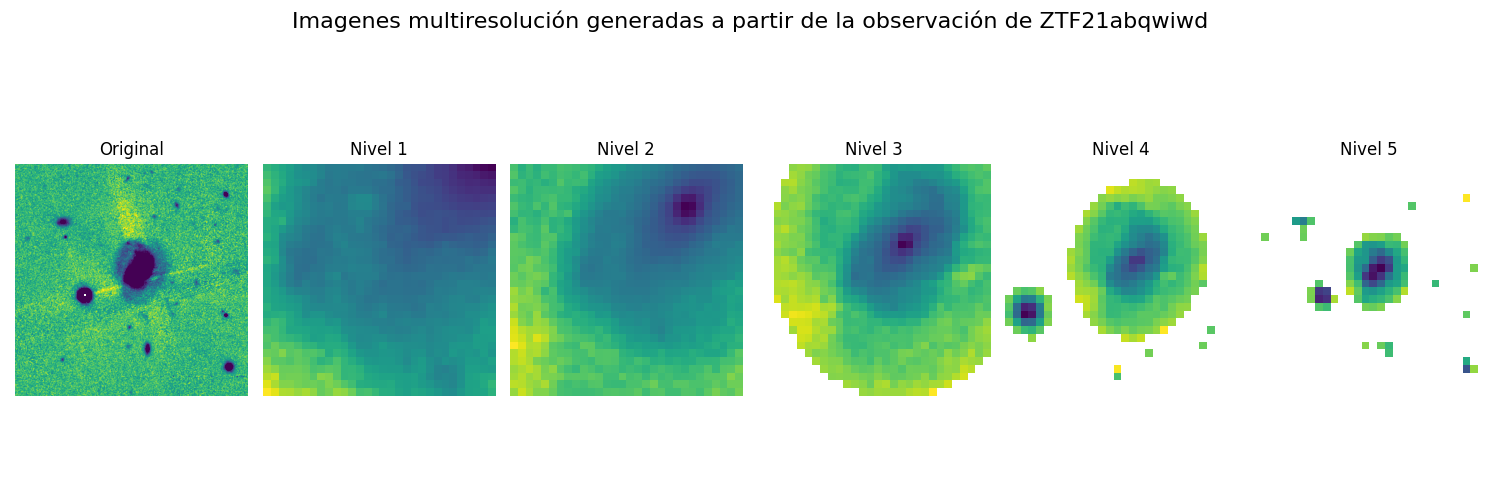
\includegraphics[width=1\linewidth]{images/introduction/delight_input_example.png}
    \caption{Imágenes multiresolución generadas a partir de la observación de la supernova \textit{ZTF21abqwiwd}, donde la primera imagen corresponde a la observación original obtenida desde el telescopio Pan-STARRS \cite{panstarrs}, y las imágenes siguientes representan las cinco resoluciones generadas.}
    \label{fig:delight-input}
\end{figure}

A la entrada le sigue una sección de \textit{Data Augmentation}, con el objetivo de dotar al modelo de robustez e invariación ante transformaciones de la imagen. Ésto se consigue realizando una transformación para cada resolución inicial, donde se generan ocho imágenes que representan las posibles rotaciones y volteos de la imagen. En total, cuarenta imágenes se generan a partir de las cinco iniciales.\par\null\par

\begin{figure}[ht!]
    \centering
    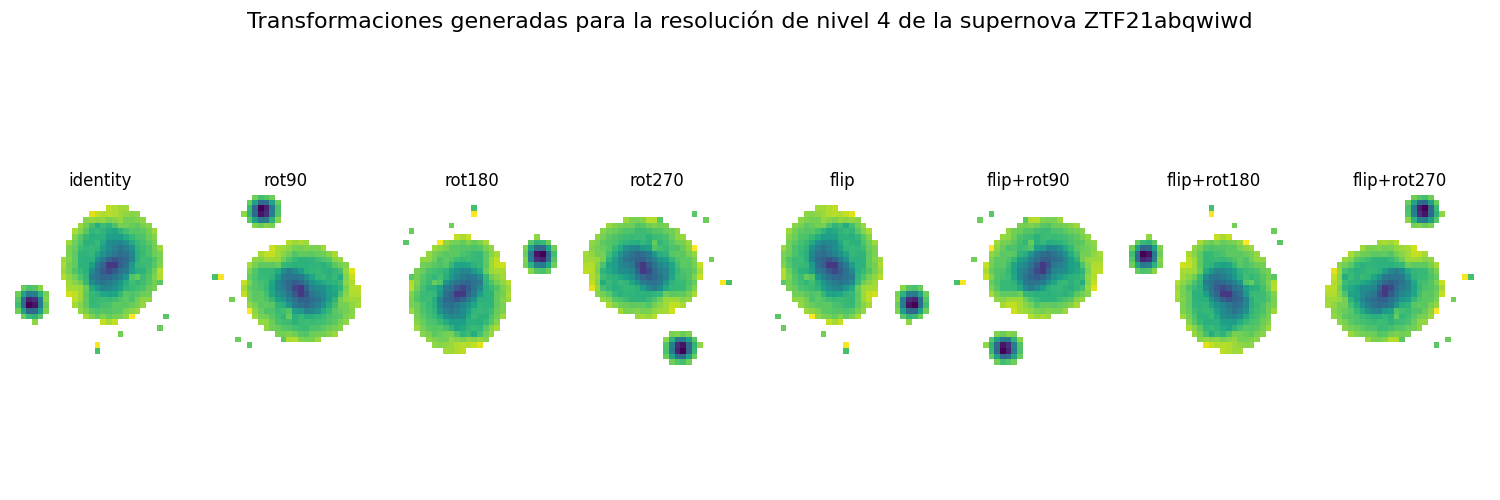
\includegraphics[width=1\linewidth]{images/introduction/delight_data_augmentation.png}
    \caption{Visualización gráfica del Data Augmentation que se genera a partir de una imagen, en el que se generan ocho imágenes resultantes. Esta transformación se aplica a cada una de las cinco resoluciones de la entrada. Las transformaciones ilustradas basadas en una imagen inicial, en orden, son: Identidad, Rotación 90°, Rotación 180°, Rotación 270°, Volteo Horizontal, Volteo Horizontal con Rotación 90°, Volteo Horizontal con Rotación 180°, y Volteo Horizontal con Rotación 270° }
    \label{fig:delight-transformation-layer}
\end{figure}

Cada una de las cuarenta imágenes es procesada en una segunda sección de carácter convolucional, compuesta por un dos capas que se componen de una convolución de kernel $3\times3$ con función de activación ReLU, seguida de un max pool con kernel $3\times3$, y una capa convolucional similar pero sin max pool, finalizando con el aplanamiento de la salida de estas convoluciones, siendo ésta ultima transformación el vector de características que representa a la imagen inicial. Todas las imágenes son procesadas por la misma sección convolucional, es decir, dicha sección comparte los pesos.\par\null\par

\begin{figure}[h]
    \centering
    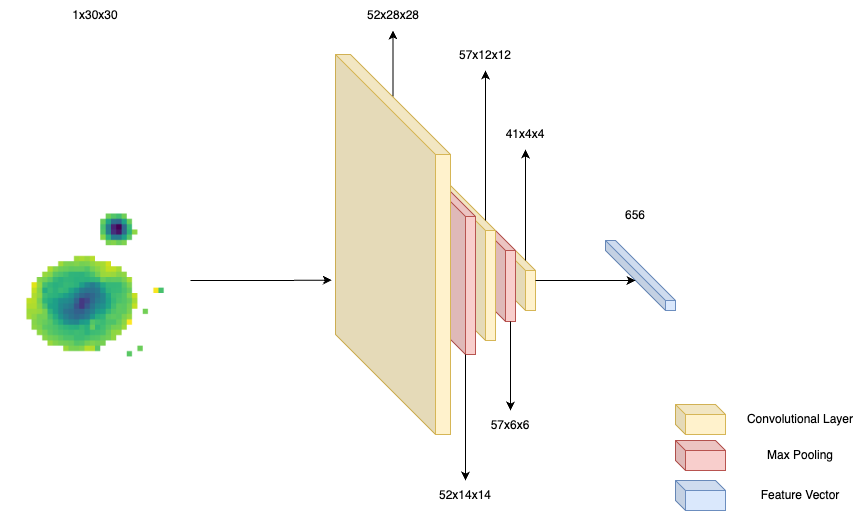
\includegraphics[width=0.63\linewidth]{images/introduction/delight_convolutional_section.png}
    \caption{Explicación gráfica de la sección convolucional, donde los cuboides amarillos representan las convoluciones, y los cuboides rojos las operaciones de max pooling. Como entrada, la sección convolucional recibe una imagen de $1\times30\times30$ y retorna un vector de características de tamaño $656$}
    \label{fig:delight-convolution-layer}
\end{figure}

Finalmente, una tercera sección procesa los vectores de características para generar el vector posición final, representando una regresión. Para esto, se concatenan cinco vectores de características correspondiente a las resoluciones de una imagen, resultando en un vector de dimensión $B\times 3280$, y se procesan en dos capas \textit{Fully Connected}, de dimensiones $B\times 3280\times 685$ y $B\times 685\times 2$, respectivamente, siendo la última de ellas una salida que representa el vector posición de la galaxia anfitriona para cada una de las transformaciones aplicadas en la primera sección, por lo que el vector de salida es de dimensión $B\times(8\cdot2)$.\par\null\par

Todo lo anterior se puede resumir en la siguiente figura extraída del trabajo original del equipo \textit{ALeRCE} \cite{delight}.\par\null\par

\begin{figure}[ht!]
    \centering
    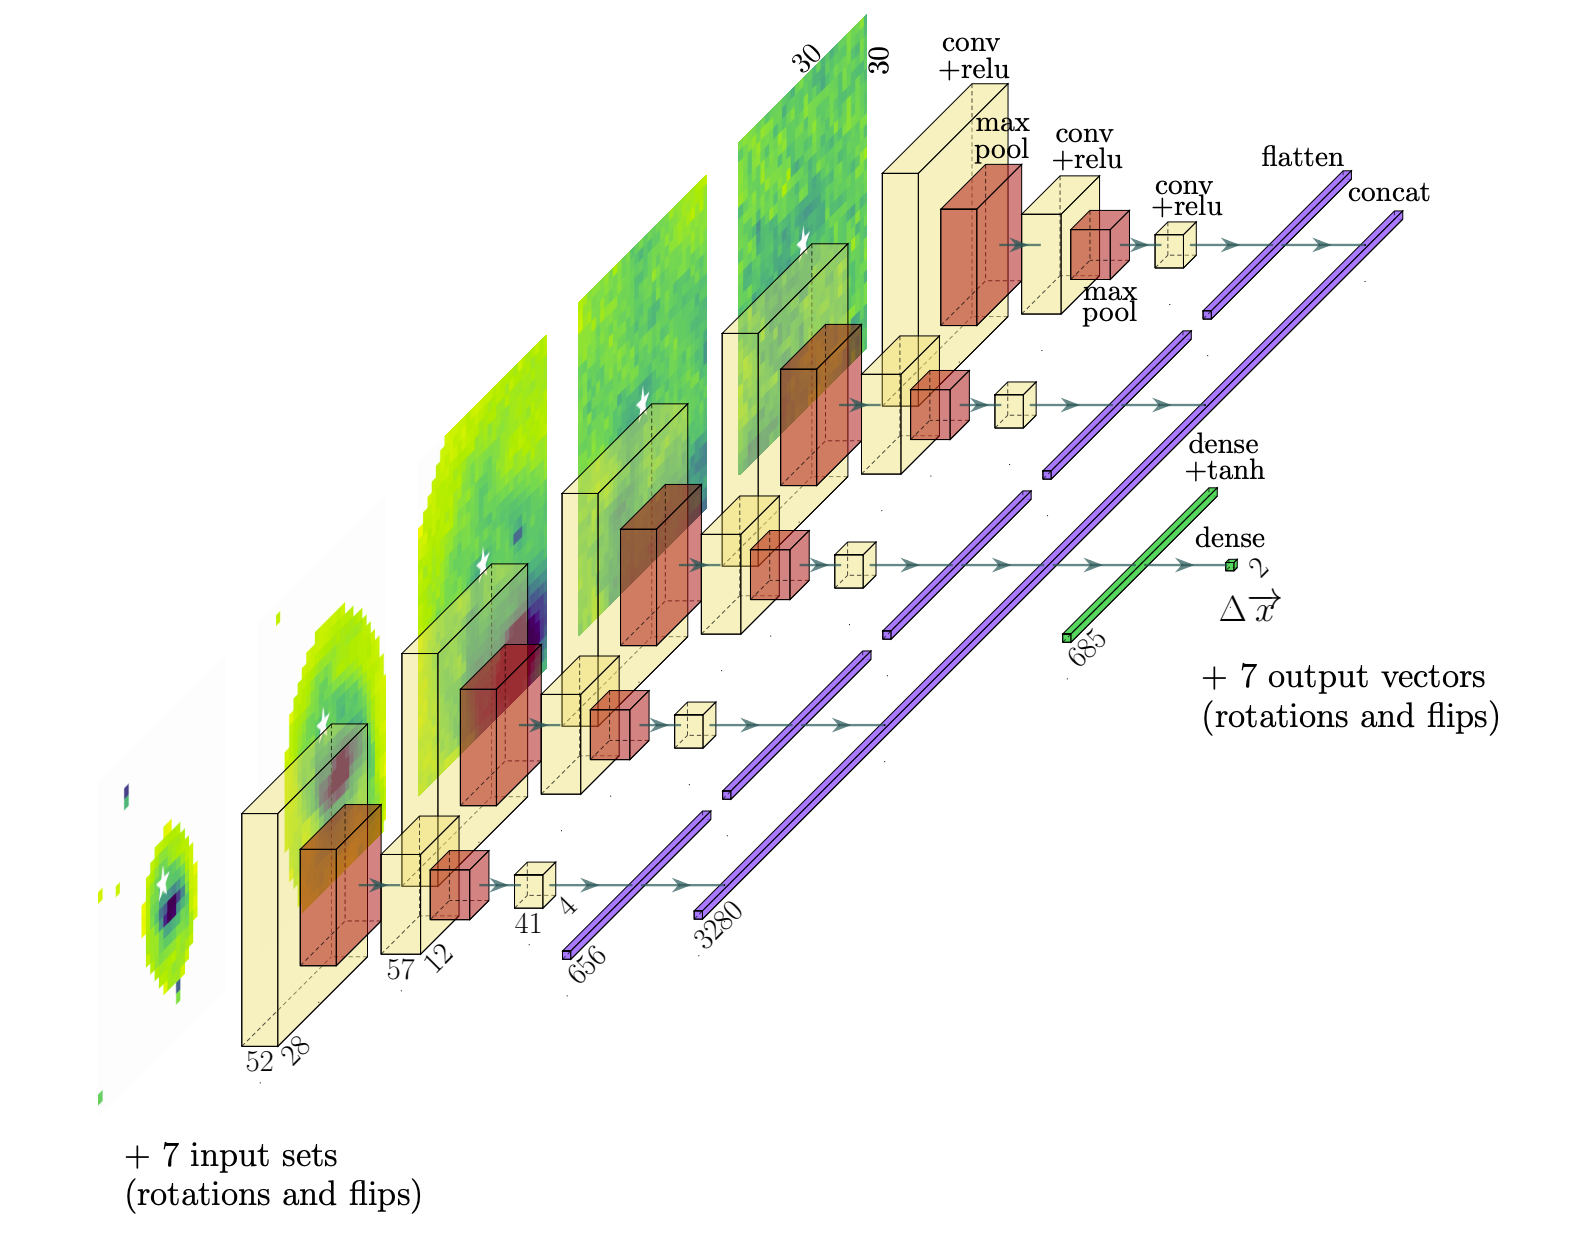
\includegraphics[width=0.7\linewidth]{images/introduction/delight_full_arch.png}
    \caption{Arquitectura completa del algoritmo DELIGHT, donde recibe cinco resoluciones de una imagen, de las cuales se generan ocho transformaciones por cada resolución dando un total de cuarenta imágenes, se generan vectores de características por cada una de las imágenes generadas, y se computan ocho posiciones, correspondiente a cada transformación realizada}
    \label{fig:delight-full}
\end{figure}

La predicción de la posición de la galaxia anfitriona se realiza promediando las ocho posiciones resultantes.\par\null\par

Las ventajas de éste método son múltiples, donde se destaca que, actualmente, es el método más rápido y preciso para la tarea de identificación de galaxias anfitrionas, abriendo paso para ser un algoritmo candidato a ser usado en el procesamiento de los datos del Legacy Survey of Space and Time (LSST) en tiempo real.\par\null\par

Sin embargo, aún quedan varios caminos por explorar; se deben explorar arquitecturas que incorporen otras fuentes de datos, como curvas de luz o información de varias bandas. También respecto al método \textbf{DELIGHT}, el procesamiento de imágenes provenientes de otros telescopios podría empeorar el desempeño del algoritmo, lo que obligaría al reentrenamiento para cada nueva fuente de datos. A su vez, el método sugiere, en el campo multimodal, la incorporación de información de varias bandas. Por lo que este trabajo abre camino a éstas interrogantes. \par\null\par

\section{Multimodalidad} \label{introduction:multimodality}
% ¿Qué es la multimodalidad?
% ¿Como la multimodalidad podría ayudar al problema de clasificación?
% ¿Por qué esto solucionaría uno de los contras del método DeLIGHT?
El uso de diversas fuentes de datos astronómicos de distinto tipo en modelos de machine learning, como las mencionadas en la sección anterior, encuentran su campo de estudio en la multimodalidad.\par\null\par

En el trabajo de \cite{multimodality} se desarrolla el marco teórico con las definiciones, conceptos claves y desafíos a abordar en el campo de la incorporación de datos de distintas fuentes a modelos de machine learning.\par\null\par

\subsection{Definición y Conceptos Clave}

La modalidad se define como \textit{una forma en que un fenómeno natural es percibido o expresado. Por ejemplo, las modalidades incluyen el habla y el audio grabados a través de micrófonos, las imágenes y los videos capturados mediante cámaras, y la fuerza y las vibraciones capturadas mediante sensores.} \cite{multimodality}. Las modalidades viven en una dimensión que representa datos desde lo más bruto a lo más abstracto. Una modalidad bruta se define como aquel dato de un fenómeno que se haya generado cerca de un sensor (dato en bruto). En cambio, las modalidades abstractas son lo contrario, haciendo referencia a razonamiento sobre datos más brutos, como el sentimiento de un audio de voz, la cantidad de objetos detectados en una imagen, etc.\par\null\par

Por lo tanto, la multimodal se refiere a \textit{situaciones donde están involucradas múltiples modalidades}. Ahora bien, desde un pusto de vista de investigación, la multimodalidad implica el estudio computacional de modalidades que cumplen tres principios específicos: \textbf{heterogeneidad}, \textbf{conectabilidad} e \textbf{interactibilidad} (interconectabilidad). Una modalidad heterogénea implica que la información presente en diferentes modalidades a menudo muestra diversas cualidades, estructuras y representaciones. Estas modalidades no son independientes, sino que comparten conexiones debido a la información complementaria entre ellas. Por último las modalidades interactúan de diferentes maneras cuando se integran para una tarea. A continuación se desglosará cada principio.\par\null\par

La \textbf{heterogeneidad} se manifiesta en múltiples dimensiones, tales como la \textbf{representación} de elementos, donde cada modalidad comprende unidades básicas de datos, como caracteres en texto o fotogramas en videos. También se observa en la \textbf{distribución}, que se refiere a las frecuencias y probabilidades de ocurrencia de estos elementos. Es posible descubrirlo en la \textbf{estructura}, que destaca cómo se componen los elementos para formar modalidades completas, como la estructura espacial en imágenes o la jerárquica en el lenguaje. Además, la heterogeneidad incluye las diferencias en el contenido de información y en los niveles de \textbf{ruido} presentes en cada modalidad, así como la \textbf{relevancia} específica de cada modalidad para tareas y contextos determinados.\par\null\par

Entender y modelar esta heterogeneidad es aplicable tanto en el análisis unimodal como multimodal. En el caso de los datos unimodales, se diseñan \textit{encoders} especializados para extraer las características únicas de cada modalidad. Para los datos multimodales, abordar la heterogeneidad permite aprender representaciones y alinear las diferentes modalidades de manera efectiva, lo cual es esencial para la integración y el análisis conjunto de múltiples fuentes de datos. Este enfoque no solo mejora la precisión y la utilidad de los modelos multimodales, sino que también aborda desafíos clave en la cuantificación y comparación de estos modelos.\par\null\par

La \textbf{conectividad} se puede entender desde perspectivas tanto estadísticas como semánticas. Desde un enfoque estadístico, las conexiones se identifican mediante patrones de distribución en los datos multimodales, mientras que los enfoques semánticos se basan en el conocimiento del dominio sobre cómo las modalidades comparten y contienen información única.\par\null\par

La perspectiva estadística se refiere a la relación entre los valores de diferentes variables, como la distribución conjunta de elementos que resulta en correlaciones. La dependencia estadística profundiza en entender el tipo exacto de dependencia entre elementos, que puede ser causal, espacial o temporal. Estas asociaciones y dependencias ayudan a modelar las distribuciones conjuntas y alinear las modalidades.\par\null\par

La perspectiva semántica trata de identificar elementos en diferentes modalidades que comparten el mismo \textit{significado}. Las relaciones semánticas van más allá de las correspondencias directas, describiendo la naturaleza de las relaciones entre elementos de distintas modalidades, ya sea semántica, lógica, causal o funcional. La identificación de éstas relaciones requiere de conocimiento del dominio en el que se esté trabajando para deducir el cómo las modalidades comparten y contienen información única.\par\null\par

Finalmente, la \textbf{interactibilidad} hace referencia a la forma en que los elementos de diferentes modalidades interactúan y se combinan para generar nueva información cuando se integran con el propósito de inferir tareas. A diferencia de las conexiones que existen de manera inherente en los datos multimodales, las interacciones solo surgen cuando las modalidades se procesan juntas para producir una nueva respuesta. Estas interacciones pueden involucrar información compartida, única o sinérgica, y pueden ser redundantes si se basan en información común a ambas modalidades, o no redundantes si se apoyan en diferentes proporciones de información compartida y única.\par\null\par

Los mecanismos de interacción abarcan operadores funcionales tanto estadísticos como semánticos, que incluyen formas aditivas, no aditivas y no lineales, así como operaciones lógicas, causales o temporales. Además, la respuesta inferida de estas interacciones puede variar; puede ser una equivalencia si la respuesta multimodal es similar a la de cualquiera de las modalidades, una mejora si la respuesta multimodal muestra mayor confianza, o puede involucrar modulaciones y emergencias, resultando en respuestas multimodales distintas a las unimodales. Este enfoque integral es crucial para entender y aprovechar la complejidad y riqueza de los datos multimodales en diversas aplicaciones.\par\null\par

\subsection{Desafíos técnicos a considerar en la multimodalidad}
El trabajo de \cite{multimodality} propone seis desafíos a considerar a la hora de trabajar con multimodalidad; la representación, la alineación, el razonamiento, la generación, la transferencia y la cuantificación. En el contexto de éste trabajo, los desafíos principales a considerar son la \textbf{representación} y \textbf{transferencia}. \par\null\par

\subsubsection{Representación}
La \textbf{representación} implica la tarea de aprender representaciones que puedan reflejar adecuadamente las interacciones entre elementos de diferentes modalidades, como texto, imágenes y audio. Este desafío se descompone en tres subcategorías principales: fusión de representaciones, coordinación de representaciones y fisión de representaciones.\par\null\par

\begin{itemize}
    \item \textbf{Fusión de representaciones:} Se centra en combinar información de múltiples modalidades para formar una representación conjunta. Esto se puede hacer a niveles abstractos, donde primero se capturan representaciones generales de cada modalidad antes de fusionarlas, o a niveles más brutos, donde la fusión se realiza en etapas tempranas utilizando datos sin procesar. Los métodos utilizados incluyen interacciones aditivas y multiplicativas, productos tensoriales y unidades de atención, que permiten capturar de manera efectiva las interacciones entre modalidades.
    \item \textbf{Coordinación de representaciones:} Busca mejorar la contextualización multimodal sin reducir el número de representaciones. Esto se logra a través de la coordinación fuerte, que alinea elementos semánticamente equivalentes en un espacio de representación, y la coordinación parcial, que captura conexiones generales como correlaciones y jerarquías. La coordinación fuerte utiliza métodos como el aprendizaje contrastivo y el mapeo de datos entre modalidades, mientras que la coordinación parcial puede incluir enfoques como el análisis de correlación canónica y el aprendizaje de jerarquías.
    \item \textbf{Fisión de representaciones:} Implica descomponer las representaciones en conjuntos más detallados que reflejan el conocimiento sobre la estructura interna de los datos multimodales. A nivel de modalidad, esto significa separar la información específica de cada modalidad de la información redundante multimodal. La fisión fina va más allá al descomponer los datos en subespacios individuales, utilizando técnicas como el clustering y la factorización de matrices.
\end{itemize}

\subsubsection{Transferencia}
La \textbf{transferencia} se enfoca en el traspaso de conocimiento entre modalidades para mejorar la precisión y robustez de los modelos, especialmente cuando una de las modalidades principales tiene datos limitados o ruidosos. Este desafío se aborda a través de tres subcategorías principales: transferencia entre modalidades, coaprendizaje multimodal e inducción de modelos.\par\null\par

La transferencia entre modalidades implica utilizar modelos entrenados en una modalidad secundaria, que puede tener más datos o ser más fácil de anotar, para ayudar a un modelo en la modalidad primaria. Este enfoque puede incluir:\par\null\par

\begin{itemize}
    \item \textbf{Ajuste de modelos preentrenados:} Modelos como los transformers, que han sido preentrenados en grandes conjuntos de datos de texto, pueden ser ajustados para tareas multimodales como la generación de descripciones de imágenes. Métodos como el ajuste de prefijo y el ajuste de representación permiten adaptar estos modelos a nuevas modalidades.
    \item \textbf{Aprendizaje multitarea:} Utiliza múltiples tareas a gran escala para mejorar el rendimiento en tareas individuales. Modelos como Perceiver y PolyViT pueden manejar múltiples modalidades y tareas simultáneamente, mejorando la capacidad del modelo para generalizar a nuevas tareas y modalidades.
    \item \textbf{Aprendizaje por transferencia:} Extiende el concepto de transferencia dentro de una misma modalidad a la transferencia entre diferentes modalidades. Por ejemplo, un modelo preentrenado en texto puede ser transferido para trabajar con imágenes o video, facilitando el aprendizaje en modalidades con menos datos.
\end{itemize}

El coaprendizaje multimodal se centra en compartir espacios de representación entre modalidades para transferir información útil. Esto puede implicar:\par\null\par

\begin{itemize}
    \item \textbf{Coaprendizaje mediante representación:} Crear un espacio de representación conjunto que utilice tanto la modalidad primaria como la secundaria durante el entrenamiento. Esto puede implicar el uso de técnicas como el aprendizaje contrastivo o la coordinación de espacios de representación para mejorar tareas específicas, como la clasificación de imágenes utilizando textos asociados.
    \item \textbf{Coaprendizaje mediante generación:} Generar una modalidad secundaria a partir de la modalidad primaria para enriquecer las representaciones de la modalidad primaria. Por ejemplo, traducir texto a imágenes o audio para mejorar la comprensión y predicción en la modalidad principal.
\end{itemize}

La inducción de modelos mantiene los modelos unimodales separados pero induce comportamientos en cada modelo utilizando la información de la modalidad secundaria. Ejemplos incluyen:\par\null\par

\begin{itemize}
    \item \textbf{Cotraining (coentrenamiento):} Entrenar dos algoritmos de aprendizaje por separado en cada vista de los datos, permitiendo que cada modelo se beneficie de la información adicional proporcionada por la otra modalidad. Este enfoque mejora la robustez y precisión de cada modelo individual.
    \item \textbf{Coregularización:} Aplicar restricciones adicionales que incentiven a los modelos unimodales a compartir información útil entre sí durante el proceso de aprendizaje, mejorando la capacidad de generalización del modelo.
\end{itemize}

\subsection{Relación entre la multimodalidad y la astronomía}
En el campo de la astronomía, la multimodalidad cobra relevanciar debido a la gran cantidad de datos disponibles a través de diversos telescopios. La multimodalidad, utilizando datos de imágenes de distintas bandas, puede mejorar la precisión de la predicción de las galaxias anfitrionas de transitorios.

\subsubsection{Uso de datos de imágenes de distintas bandas}
Las imágenes obtenidas de diferentes bandas (grizy) del PanSTARRS \cite{panstarrs}, ofrecen información complementaria sobre las galaxias. Cada banda puede revelar diferentes características físicas y químicas del objeto observado. Por ejemplo, la banda g puede ser más sensible a la luz de las estrellas jóvenes y calientes, mientras que la banda z puede penetrar mejor a través del polvo interestelar y revelar estructuras ocultas.\par\null\par

Al integrar estas diversas fuentes de datos, los modelos pueden aprender a identificar patrones y correlaciones que no serían evidentes utilizando una sola banda. Este enfoque multimodal es esencial para mejorar la precisión y robustez de los modelos de identificación de galaxias anfitrionas, permitiendo una caracterización más completa y precisa de los eventos transitorios.\par\null\par

El modelo \textbf{DELIGHT} \cite{delight}, como se propone en la introducción de esta tesis, es una herramienta innovadora diseñada para abordar el problema de la identificación de galaxias anfitrionas utilizando imágenes multiresolución. Aunque inicialmente se centró en la banda r del PanSTARRS, el potencial de \textbf{DELIGHT} puede ser ampliado incorporando datos de múltiples bandas, alineándose con los principios de la multimodalidad.\par\null\par

Ésto es posible modificando la entrada del modelo para aceptar un tensor que incluya las diferentes bandas como canales adicionales, rescatando la estrategia de la representación como fusión analizado en la sección anterior. El procesamiento de estas bandas permitirá al modelo aprender de una representación más detallada de los datos, y así, mejorar las métricas de rendimiento del modelo, tales como la precisión, la tasa de falsos positivos y la capacidad de generalización. 

\newpage

\section{Objetivos} \label{introduction:objectives}
\subsection{Objetivo General}

\paragraph{Desarrollar modelos de identificación de galaxias con entrada de imágenes multiresolución estudiando el desempeño, tanto en velocidad de procesamiento como en correctitud en la tarea a resolver.}

\subsection{Objetivos Específicos}
\begin{itemize}
    \item Explorar la extensión multi modal y multi tarea , e.g. incorporar información de varias bandas, o la serie de tiempo asociada al transitorio, o las imágenes referencia, ciencia y diferencia con las que se descubrió el transitorio; resolver el problema de identificación de la galaxia y clasificación del transitorio usando los mismos datos.
    \item Explorar la fiabilidad del algoritmo para otras fuentes de datos.
    \item Identificar casos problemáticos, e.g. cuando el modelo no puede elegir entre dos galaxias, y explorar soluciones.
\end{itemize}

\end{document}
